
\begin{table*}[ht!]
\centering
{\small
\begin{tabular}{l@{\hspace{2cm}}cc@{\hspace{1cm}}cc@{\hspace{1cm}}c} \hline
       & \multicolumn{5}{c}{{\bf System Performance: Rouge-1}}\\
       & \multicolumn{5}{c}{{\bf Gold Standard: Historical Notes}}\\ \hline
Method & {\bf  src} & 95\% C.I. & {\bf cit} & 95\% C.I. & Mean\\ \hline \hline
{\bf LexRank}                   & 0.150 & [0.110, 0.190]  & 0.212 & [0.189, 0.235]  & 0.181\\
{\bf C-LexRank}                 & 0.183 & [0.147, 0.220]  & 0.187 & [0.158, 0.217]  & 0.185\\
{\bf HITS}                      & 0.202 & [0.162, 0.243]  & 0.152 & [0.120, 0.185]  & 0.177\\
{\bf HITS with weights}         & {\bf 0.216} & {\bf [0.195, 0.237]}  & 0.200 & [0.178, 0.222]  & 0.208\\
%{\bf HITS with priors}          & 0.207 & [0.182, 0.233]  & 0.138 & [0.100, 0.177]  & 0.173\\
{\bf HITS with weights/priors}  & 0.204 & [0.187, 0.221]  & {\bf 0.215} & {\bf [0.181, 0.249]}  & {\bf 0.209}\\ \hline 
\end{tabular}}
\caption{Average Rouge-1 scores of automatic surveys of the 10 chapters listed in Table~\ref{tbl:chapters} evaluated using historical notes as reference (C.I.: Confidence Interval).}\label{tbl:rouge1-hist}
\end{table*}

\section{Experiments}
\label{sec:exp}

Using the procedure described in section~\ref{sec:hist}, we extract the list of source papers from 10 chapters' historical notes in the JM book. For each chapter, the papers cited in its historical note are used as the source papers ({\bf src}) and the set of AAN papers that cite them are used as citing papers ({\bf cit}). 
Table~\ref{tbl:chapters} summarizes the list of chapter historical notes used in our experiments together with the number of source papers,  citing papers extracted from AAN, the size of the left ($\B_L$) and right ($\B_R$) components in the bi-partite graph, and number of edges in the graph ($E_\B$).

For each chapter we generate $2\times 2$ summaries using the {\bf cit} and {\bf src} papers with a length equal to the length of chapter's {\bf chapter summaries} and that of chapter's {\bf historical notes}. We evaluate these summaries using Rouge~\cite{Lin2004}, and compare them with two state-of-the-art methods in scientific survey generation: LexRank and C-LexRank.

\subsection{Baseline Methods}
\vspace{-2mm}
\subsubsection{LexRank}
LexRank~\cite{Erkan&Radev04c} works by first building a graph of all
the documents ($D_i$) in a cluster. The edges between corresponding nodes ($d_i$) represent
the cosine similarity between them if the cosine value is above a threshold (0.10 following~\cite{Erkan&Radev04c}).  
Once the network is built, the system finds the most central sentences
by performing a random walk on the graph. 

{\small
\begin{eqnarray}\label{eqn:3}
p(d_j) = (1- \lambda) \frac{1}{|D|}+ \lambda\sum_{d_i}p(d_i)P(d_i\rightarrow d_j) 
\end{eqnarray}}

\subsubsection{C-LexRank}
C-LexRank is a clustering-based summarization system that is proposed by \cite{Qazvinian&Radev08a} to summarize different scientific perspectives. create a full connected network in which nodes are sentences and edges are cosine similarities.  
To create summaries, C-LexRank constructs a fully connected network in which vertices are sentences and edges are cosine similarities calculated using the TF-IDF vectors of citation sentences. 
It then employs a hierarchical agglomeration clustering algorithm proposed by \cite{Clauset04} to find communities of sentences that discuss the same scientific contributions.

Once the graph is clustered and communities are formed, \newcite{Qazvinian&Radev08a} extract sentences from different clusters to build a summary.  
They start with the largest cluster and extract sentences using LexRank within each cluster.
In other words, for each cluster $\Omega_i$ they make a lexical network of \emph{the sentences in that cluster} ($N_i$). 
LexRank  extracts the most central sentences in $N_i$ as salient sentences of $\Omega_i$ to include in the main summary. 
For each cluster $\Omega_i$, the most salient sentence of $\Omega_i$ is extracted until the summary length limit is reached. The cluster selection is in order of decreasing size.

\subsection{Results and Discussion}
Table~\ref{tbl:rouge1-hist} lists the average Rouge-1 scores of different automatic summaries with each chapter's {\bf historical notes} chosen as the gold standard and its length as the automatic summary length. Similarly, Table~\ref{tbl:rouge1-summ} summarizes the average Rouge-1 scores of different system summaries when {\bf chapter summaries} are used as reference.

\begin{table*}[ht!]
\centering
{\small
\begin{tabular}{l@{\hspace{2cm}}cc@{\hspace{1cm}}cc@{\hspace{1cm}}c} \hline
       & \multicolumn{5}{c}{{\bf System Performance: Rouge-1}}\\
       & \multicolumn{5}{c}{{\bf Gold Standard: Chapter Summaries}}\\ \hline
Method & {\bf  src} & 95\% C.I. & {\bf cit} & 95\% C.I. & Mean\\ \hline \hline
{\bf LexRank}                   & 0.205 & [0.141, 0.269]  &  0.232 & [0.203, 0.260]  & 0.218 \\
{\bf C-LexRank}                 & 0.188 & [0.129, 0.246]  &  0.198 & [0.140, 0.256]  & 0.193 \\
{\bf HITS}                      & 0.233 & [0.191, 0.274]  &  0.161 & [0.122, 0.200]  & 0.197 \\
{\bf HITS with weights}         & {\bf 0.242} & {\bf [0.215, 0.268]}  &  0.222 & [0.183, 0.260]  & 0.232 \\
%{\bf HITS with priors}          & 0.205 & [0.170, 0.239]  &  0.129 & [0.094, 0.165]  & 0.167 \\
{\bf HITS with weights/priors}  & 0.235 & [0.198, 0.271]  &  {\bf 0.241} & {\bf [0.198, 0.284]}  & {\bf 0.238} \\ \hline
\end{tabular}}
\caption{Average Rouge-1 scores of automatic surveys of the 10 chapters listed in Table~\ref{tbl:chapters} evaluated using chapter summaries as reference (C.I.: Confidence Interval).}\label{tbl:rouge1-summ}
\end{table*}

\begin{table}
\centering
{\scriptsize
\begin{tabular}{p{1cm}p{6cm}} \hline
\multicolumn{2}{c}{{\bf Part of the automatic summary}}\\ \hline
early developments & {\it During the early stages of the Penn Treebank project, the initial automatic POS assignment was provided by PARTS (Church 1988), a stochastic algorithm developed at AT\&T Bell Labs.}\\ [1.5ex]
methods & {\it As shown by Klein and Manning (2002, 2004), the extension to inducing trees for words instead of p-o-s tags is rather straight-forward since there exist several unsupervised part-of-speech taggers with high accuracy, which can be combined with unsupervised parsing (see e.g. Schutze 1996; Clark 2000).}\\ [1.5ex]
ambiguity problem &  {\it Jardino and Adda (1994), Schutze (1997) and Clark (2000) have attempted to address the ambiguity problem to a certain extent.}\\ \hline
\end{tabular}}
\caption{Part of the automatic survey generated using {\bf HITS with weights} for ``part-of-speech tagging'' signifying early work, state-of-the-art, etc. (The labels are manually extracted for better illustration of the summary quality, and are not a by-product of the system)}\label{tbl:outeg}
\end{table}

Both of these tables show that in general the HITS method that employs weights on graph edges leads to significantly better results than other methods both when the summaries are generated from citations (cit) or source texts (src). Moreover, these tables suggest that the HITS method when employing weights and priors outperforms the state-of-the-art methods and baselines when summaries are generated using  citations (cit).
Table~\ref{tbl:outeg} shows part of the automatic survey generated using {\bf HITS with weights} for ``part-of-speech tagging'' signifying some early work, state-of-the-art, etc. For better illustration of the quality of this survey, we have manually labeled each sentence with its role (i.e., early developments, methods, etc.)

We repeat the same experiments using Rouge-L. Figure~\ref{fig:rougel} summarizes the average Rouge-L score for automatic summaries generated using source texts (src) and citations (cit). This figure confirms that Rouge-L results follow a similar pattern as Rouge-1. 
The results in Figure~\ref{fig:rougel} and Tables~\ref{tbl:rouge1-summ},~\ref{tbl:rouge1-hist} also suggest that surveys generated using citations are consistently better that those generated from source texts in LexRank and C-LexRank. However, when the two summaries are generated using both sources affecting each other in a bi-partite graph, summaries from source and citations obtain similar qualities on average.

In summary, we observe that using semantic relatedness and adding weights to the bi-partite citation graph increases the quality of the produced summaries. One explanation is that weights enforce citation sentences (source sentences) to obtain high scores only when they are connected to important source sentences (citation sentences) that are also semantically similar  similar to them. 

\begin{figure}
\centering
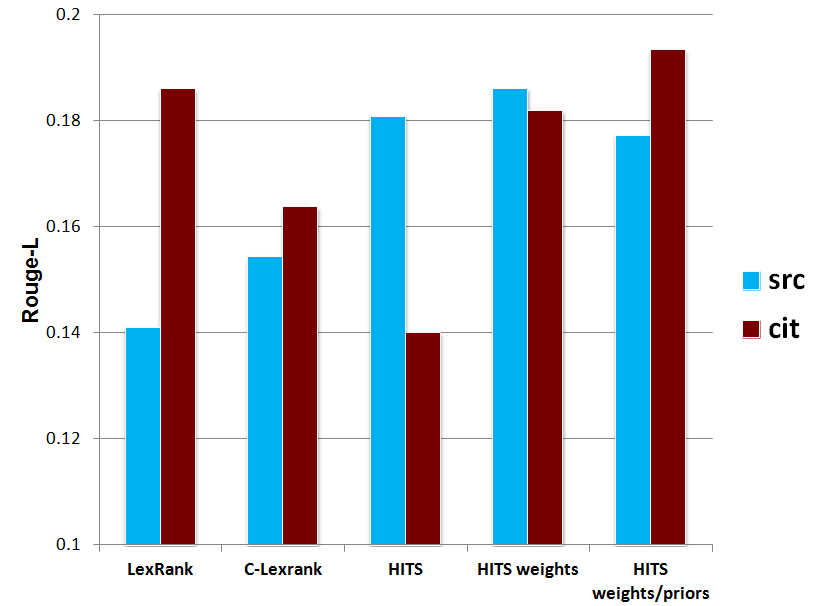
\includegraphics[width=\columnwidth]{images/rougel-2}
\caption{Average Rouge-L scores of automatic surveys of the 10 chapters listed in Table~\ref{tbl:chapters}  using chapter summaries and historical notes as reference }\label{fig:rougel}
\end{figure}


\subsection{Nugget-based Evaluations}
In addition to Rouge, we evaluate the quality of the automatic summaries using the \emph{pyramid score}. This evaluation metric relies on human judgments and manual nugget annotations~\cite{jimmy06,nenkova2004ecs,Wesley:2004,Vorhees:2003}. In pyramid evaluation, different factoids \cite{vahed&radev2011} obtain different weights, and the quality of a summary is measured using the F-measure calculated from its factoid recall and  precision values. 

In order to evaluate the performance of the proposed graph-based algorithm with respect to human extracted nuggets, we use the QA dataset from~\cite{mohammad-EtAl:2009:NAACLHLT09}. In their work, \newcite{mohammad-EtAl:2009:NAACLHLT09} performed their experiments on  a set of papers in the research area of Question Answering (QA).
They selected the papers in each corpus by matching the phrases ``Question Answering'' in the title and the content of AAN papers. The QA dataset contains 10 papers cited in 146 sentences from 62 papers in AAN.

\newcite{mohammad-EtAl:2009:NAACLHLT09} created a set of gold standards for the QA data from citation texts and abstracts, respectively.
They asked three human judges to identify important nuggets of information worth including in a survey from QA citations and QA abstract.
More particularly, they instruct annotators to extract prioritized lists of 2--8 nuggets from abstracts and citations of each paper. These lists are them merged to build the pyramid model that can be used to evaluate automatically generated summaries.

We use this dataset to evaluate the performance of the HITS algorithm using the nugget-based pyramid method. We obtain the citations and the nuggets for the QA papers, which were extracted from AAN's 2009 release. 
We also obtained the source text of the QA papers from the most recent AAN papers to build the graph. 
Since the nuggets that were extracted by \newcite{mohammad-EtAl:2009:NAACLHLT09} were from citations and abstracts, and that our source papers may not be identical to the original set, we only evaluate automatic summaries that are generated using citations in this section, and not the full-text.

When evaluated on this data, the HITS algorithm outperforms LexRank and C-LexRank. Table~\ref{tab:nugget} shows that the summaries generated using  the HITS model that employs weights on network edges produces higher quality summaries that LexRank and C-LexRank as well as the  Random summarizer, which pick sentences from citation sets randomly.

\begin{table}
{\small
\centering
\begin{tabular}{l cc}
\hline
\multicolumn{3}{c}{\bf System Performance: Pyramid F-measure}\\ \hline
& \multicolumn{2}{c}{\bf Nuggets:}\\ 
System & QA--CT & QA--AB\\ \hline \hline
{\bf Random}                    & 0.321 & 0.395\\
{\bf LexRank}                   & 0.295 & 0.320\\
{\bf C-LexRank}                 & 0.434 & 0.388\\
{\bf HITS}                      & 0.421 & 0.347\\
{\bf HITS with weights}         & {\bf 0.474} & {\bf 0.462}\\
{\bf HITS with weights/priors}  & 0.149 & 0.101\\
\hline
\end{tabular}}
\caption{Pyramid F-measure scores of automatic surveys of QA data. The surveys are evaluated using nuggets drawn from QA citation texts (QA--CT) and QA abstracts (QA--AB).}
\label{tab:nugget}
\end{table}

